\subsection{Вычисление интегралов Лебега}

\begin{note}
	В данном параграфе мы работаем с пространством $\R^n$, которое будем рассматривать как $\R^n = \R^m \times \R^k$, $m, k \ge 1$. При этом введём следующие обозначения:
	\begin{itemize}
		\item $X := \R^m$, $Y := \R^k$
		
		\item $\mu, \mu_X, \mu_Y$ --- мера Лебега на $\R^n$, $X$, $Y$ соответственно
		
		\item $d\mu(x, y) := d\mu$
		
		\item $d\mu(x) := d\mu_X$
		
		\item $d\mu(y) := d\mu_Y$
	\end{itemize}
	Теперь понятие измеримости и <<почти всюду>> неоднозначны --- какую меру мы подразумеваем? Если $\eta$ --- это какая-то из вышеперечисленных мер, то теперь мы будем явно писать $\eta$-измеримость и <<$\eta$-почти всюду>>.
\end{note}

\begin{definition}
	\textit{Сечением множества} $A \subseteq \R^n$ называются множества такого вида:
	\begin{itemize}
		\item $A_Y(x) := \{y \in Y \such (x, y) \in A\} \subseteq Y$
		
		\item $A_X(y) := \{x \in X \such (x, y) \in A\} \subseteq X$
	\end{itemize}
\end{definition}

\begin{center}
	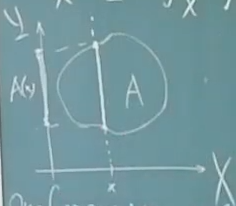
\includegraphics[width=0.4\textwidth]{images/section.png}
\end{center}

\begin{theorem} (Вычисление меры множества через меры сечений)
	Если $A \subseteq \R^n$ измеримо по Лебегу, то есть 2 симметричных свойства:
	\begin{enumerate}
		\item Для $\mu_X$-почти всех $x \in X$ сечение $A_Y(x)$ является $\mu_Y$-измеримым и имеет место равенство:
		\[
			\mu(A) = \int_X \mu_Y(A_Y(x))d\mu(x)
		\]
		
		\item Для $\mu_Y$-почти всех $y \in Y$ сечение $A_X(y)$ является $\mu_X$-измеримым и имеет место равенство:
		\[
		\mu(A) = \int_Y \mu_X(A_X(y))d\mu(y)
		\]
	\end{enumerate}
\end{theorem}

\begin{proof}
	Теорема доказывается путём разбора случаев от бруса к множеству бесконечной меры:
	\begin{enumerate}
		\item $A = \prod_{i = 1}^n \tbr{a_i; b_i}$ --- брус. Тогда, если $x \in \prod_{i = 1}^m \tbr{a_i; b_i} = B$, то как будет выглядеть сечение $A_Y(x)$?
		\[
			A_Y(x) = \prod_{j = m + 1}^n \tbr{a_j; b_j};\ \ \ \mu_Y(A_Y(x)) = \prod_{j = m + 1}^n (b_j - a_j)
		\]
		Если же $x \notin B$, то $A_Y(x) = \emptyset$. Итого:
		\[
			\int_X \mu_Y(A_Y(x))d\mu(x) = \int_{B} \prod_{j = m + 1}^n (b_j - a_j)d\mu_X = \prod_{j = 1}^n (b_j - a_j) = \mu(A)
		\]
		
		\item $A = \bigcup_{i = 1}^N C_i$ --- элементарное множество, где $C_i = \prod_{j = 1}^n \tbr{a_{i, j}; b_{i, j}}$ --- брусья, причём $\forall i \neq j\ \Int C_i \cap \Int C_j = \emptyset$.
		
		Установим индукцией по $m$, что $A = \bigcup_{j = 1}^Q P_j \times M_j$, где $P_j = \prod_{i = 1}^m \tbr{a_{i, j}; b_{i, j}}$, $M_j$ --- брусья и элементарные множества соответственно, причём все попарно непересекаются по внутренностям.
		
		\begin{center}
			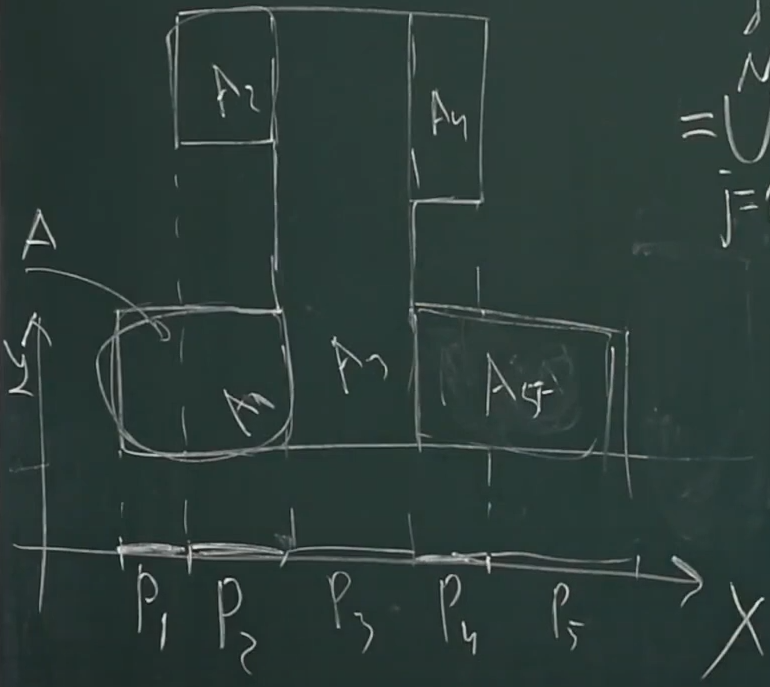
\includegraphics[width=0.4\textwidth]{images/elementary_section.png}
		\end{center}
		
		\begin{itemize}
			\item База $m = 1$: Возьмём самую левую и правую координату $X$ каждого бруса и упорядочим их: $c_1 \le \ldots \le c_M$. Тогда $A = \bigcup_{j = 1}^{M - 1} \tbr{c_j; c_{j + 1}} \times M_j$
			
			\item Переход $m > 1$: Мы уже добились размерности $m - 1$ для $P_j$. Применим рассуждения из базы к каждому $M_j$. Тогда $P_j \times M_j = \bigcup_{t = 1}^{S - 1} (P_j \times \tbr{c_t; c_{t + 1}}) \times S_t$, где $S_t$ --- одно из элементарных множеств, возникших в рассуждениях по базе. Множество в скобках будет ничем иным, как брусом размерности $m$, причём сами эти брусья попарно непересекаются по внутренностям в этой размерности. Объединяя все новые микроразбиения в одно, докажем требуемое.
		\end{itemize}
		Теперь мы имеем право заявить, что $\mu(A) = \sum_{j = 1}^Q \mu(P_j \times M_j)$ (мера границ, чья размерность меньше $m$, равна нулю). Если взять $x \in X = \R^m$, то как устроено $A_Y(x)$?
		\[
			A_Y(x) = \System{
				&{M_j,\ x \in P_j}
				\\
				&{\emptyset,\ x \notin \bigcup_{j = 1}^Q P_j}
			}
		\]
		По свойствам меры Лебега и аддитивности интеграла имеем
		\[
			\mu_Y(A_Y(x)) = \sum_{j = 1}^Q \mu_Y(M_j) \cdot \chi_{P_j}(x) \Lora \int_X \mu_Y(A_Y(x)) d\mu(x) = \sum_{j = 1}^Q \mu_Y(M_j) \mu_X(P_j) = \mu(A)
		\]
		\textcolor{red}{Как я понимаю, последний переход мы считаем интуитивно понятным и не доказываем связь $\mu, \mu_X$ и $\mu_Y$}
		
		\item $A = \bigcup_{i = 1}^\infty A_i$, где $A_i$ --- элементарные множества, $\mu(A) < +\infty$, а также $A_i \subseteq A_{i + 1}$. Про элементарные множества уже известно, что
		\[
			\mu(A_i) = \int_X \mu_Y((A_i)_Y(x))d\mu(x)
		\]
		В силу монотонности последовательности $A_i$, $A = \lim_{i \to \infty} A_i$. Стало быть, по непрерывности меры Лебега $\mu(A) = \lim_{i \to \infty} \mu(A_i)$. Аналогично $A_Y(x) = \lim_{i \to \infty} (A_i)_Y(x)$ и $\mu_Y(A_Y(x)) = \lim_{i \to \infty} \mu_Y((A_i)_Y(x))$. Заметим, что последовательность последнего предела является функциональной и даже выполнены все требования теоремы Леви:
		\[
			\Ra \int_X \mu_Y(A_Y(x))d\mu(x) = \lim_{i \to \infty} \int_X \mu_Y((A_i)_Y(x))d\mu(x) = \lim_{i \to \infty} \mu(A_i) = \mu(A)
		\]
		
		\item $A$ --- произвольное множество конечной меры. По теореме о структуре измеримых множеств
		\[
			A = \Bigg(\bigcap_{i = 1}^\infty \underbrace{\bigcup_{j = 1}^\infty A_{i, j}}_{B_i}\Bigg) \bs A_0
		\]
		Напомним, что мы знаем про множества этой цепочки:
		\begin{itemize}
			\item $A_{i, j}$ --- элементарные множества
			
			\item $\forall i, j \in \N\ \ A_{i, j} \subseteq A_{i, j + 1}$
			
			\item $\forall i \in \N\ \ B_i \supseteq B_{i + 1}$
			
			\item $\mu(B_1) < +\infty$
			
			\item $\mu(A_0) = 0$
		\end{itemize}
		Обозначим $B := \bigcap_{i = 1}^\infty B_i$. Хочется показать, что для $B$ работает эта теорема. Заметим, что есть такое равенство и свойства:
		\[
			B_1 \bs B = \bigcup_{i = 1}^\infty (B_1 \bs B_i);\ \ (B_1 \bs B_i) \subseteq (B_1 \bs B_{i + 1});\ \ \mu(B_1 \bs B_i) \le \mu(B_1) < +\infty
		\]
		С учётом верного равенства $\mu_Y((B_1 \bs B_i)_Y(x)) = \mu_Y((B_1)_Y(x)) - \mu_Y((B_i)_Y(x))$ получим требуемое:
		\begin{multline*}
			\mu(B_1) - \mu(B) = \mu(B_1 \bs B) = \lim_{i \to \infty} \mu(B_1 \bs B_i) =
			\\
			\lim_{i \to \infty} \int_X \mu_Y((B_1 \bs B_i)_Y(x))d\mu(x) = \int_X \ps{\lim_{i \to \infty} \mu_Y((B_1 \bs B_i)_Y(x))}d\mu(x) =
			\\
			\int_X \mu_Y((B_1 \bs B)_Y(x))d\mu(x) = \mu(B_1) - \int_X \mu_Y(B_Y(x))d\mu(x)
		\end{multline*}
		Остаётся аналогичным образом разобраться с $A_0$ --- применим и для него теорему о структуре измеримых множеств. Тогда найдётся $B_0 \supseteq A_0$ такое, что $\mu(B_0) = 0$ (соответствует $B$ для $A$). Для него мы уже знаем, что
		\[
			\mu(B_0) = 0 = \int_X \mu_Y((B_0)_Y(x))d\mu(x)
		\]
		В силу свойств подыинтегральной функции, это означает, что $\mu_Y((B_0)_Y(x)) = 0$ $\mu_X$-почти всюду на $X$. Так как $(B_0)_Y(x) \supseteq (A_0)_Y(x)$, то аналогичное верно и про $\mu_Y((A_0)_Y(x))$. Тогда
		\[
			\mu(A_0) = 0 = \int_X \mu_Y((A_0)_Y(x))d\mu(x)
		\]
		Собирая это всё воедино, получим итоговое равенство:
		\begin{multline*}
			\mu(A) = \mu(B \bs A_0) = \mu(B) - \mu(A_0) = \int_X \mu_Y(B_Y(x))d\mu(x) - 0 =
			\\
			\int_X \mu_Y(B_Y(x))d\mu(x) - \int_X \mu_Y((A_0)_Y(x))d\mu(x) = \int_X \mu_Y(A_Y(x))d\mu(x)
		\end{multline*}
		
		\item $A$ --- произвольное множество бесконечной меры. Тогда мы можем записать $A$ через предел неубывающей последовательности измеримых множеств конечной меры, $A = \bigcup_{i = 1}^\infty A_i$. Для каждого $A_i$ теорема уже доказана, поэтому можно написать следующее:
		\[
			A = \lim_{i \to \infty} A_i \Ra \mu(A) = \lim_{i \to \infty} \mu(A_i) = \lim_{i \to \infty} \int_X \mu_Y((A_i)_Y(x))d\mu(x)
		\]
		При этом снова $\mu_Y((A_i)_Y(x)) \le \mu_Y((A_{i + 1})_Y(x))$, $\mu_Y(A_Y(x)) = \lim_{i \to \infty} \mu_Y((A_i)_Y(x))$, посему можно применить теорему Леви и получить требуемое:
		\[
			\mu(A) = \lim_{i \to \infty} \int_X \mu_Y((A_i)_Y(x))d\mu(x) = \int_X \lim_{i \to \infty} \mu_Y((A_i)_Y(x))d\mu(x) = \int_X \mu_Y(A_Y(x))d\mu(x)
		\]
	\end{enumerate}
\end{proof}

\begin{definition}
	Пусть $f \colon E \to \ole{\R}$, $E \subseteq \R^n$ --- неотрицательная функция. Тогда \textit{подграфиком} $f$ называется множество $D_{f, E} \subseteq \R^n \times \ole{\R}$, имеющее такой вид:
	\[
		D_{f, E} = \{(x, y) \such x \in E, y \in [0; f(x)]\}
	\]
\end{definition}

\begin{lemma}
	Если $f \colon E \to \ole{\R}$, $E \subseteq \R^n$ --- неотрицательная и измеримая на $E$ функция, то её подграфик $D_{f, E}$ измерим, причём
	\[
		\mu(D_{f, E}) = \int_E f(x)d\mu(x) = \int_{[0; +\infty]} \mu(\{x \in E \colon f(x) \ge y\})d\mu(y)
	\]
\end{lemma}

\begin{proof}~
	\begin{itemize}
		\item Измеримость. Аккуратно разберём пару случаев:
		\begin{enumerate}
			\item $f$ --- ступенчатая функция. Тогда число значений $f$ не более чем счётно и подграфик можно записать в таком виде:
			\[
			D_{f, E} = \bscup_{j = 0}^\infty E_j \times [0; a_j]
			\]
			где $a_j \in f(E)$, а $E_j = \{x \in E \such f(x) = a_j\}$ --- измеримое множество (в силу измеримости $f$). $E_j \times [0; a_j]$ является цилиндрическим множеством, а поэтому измеримым (в прошлом семестре была лемма для квадрируемого основания, но её можно доказать и для измеримого по Лебегу. Для $a_0 = +\infty$ помним про $\mu(E_0) = 0$ и соглашение). Так как система измеримых по Лебегу множеств образует $\sigma$-алгебру, то $D_{f, E}$ тоже будет измеримо.
			
			\item $f$ --- произвольная функция. Коль скоро $f$ измерима по условию (тут мы говорим про измеримость без $E_0 = \{x \in E \colon f(x) = +\infty\}$), она представима равномерно сходящимся пределом неубывающих ступенчатых функций $h_m \rra f$. В силу неубывания этих функций, их подграфики образуют тоже неубывающую последовательность, сходящуюся к $D_{f, E} \bs (E_0 \times [0; +\infty])$:
			\[
				\lim_{m \to \infty} D_{f_m, E} = D_{f, E} \bs E_0 = \bigcup_{m = 1}^\infty D_{f_m, E}
			\]
			При этом каждый подграфик по предыдущему пункту измерим. Стало быть, предельный подграфик тоже измерим. Аналогично и с $D_{f, E}$ ($E_0 \times [0; +\infty]$ измеримо по соглашению)
		\end{enumerate}
	
		\item Равенство. Заметим следующие сечения $D_{f, E}$ (при соответствующих размерностях $X, Y$):
		\begin{align*}
			&{(D_{f, E})_Y(x) = [0; f(x)]}
			\\
			&{(D_{f, E})_X(y) = \{x \in E \colon f(x) \ge y\}}
		\end{align*}
		Просто применяем теорему о вычислении меры через сечения.
	\end{itemize}
\end{proof}

\begin{theorem} (Фубини)
	Пусть $E \subseteq \R^n$ --- измеримое множество, представленное в виде $E = X \times Y$, а $f \colon E \to \ole{\R}$ --- это суммируемая на $E$ функция. Тогда
	\begin{enumerate}
		\item При $\mu_X$-почти всех $x \in X$ функция $f(x, y)$ суммируема по мере $\mu_Y$ на $E_Y(x)$. И наоборот: при $\mu_Y$-почти всех $y \in Y$ функция $f(x, y)$ суммируема по мере $\mu_X$ на $E_X(y)$
		
		\item Функция $\int_{E_Y(x)} f(x, y)d\mu(y)$ суммируема на $X$, а $\int_{E_X(y)} f(x, y)d\mu(x)$ суммируема на $Y$
		
		\item Справедлива формула сведения интеграла к повторным:
		\[
			\int_E f(x, y)d\mu(x, y) = \int_X \ps{\int_{E_Y(x)} f(x, y)d\mu(y)}d\mu(x) = \int_Y \ps{\int_{E_X(y)} f(x, y)d\mu(x)}d\mu(y)
		\]
	\end{enumerate}
\end{theorem}

\begin{proof}
	Разберём случаи на $f$:
	\begin{enumerate}
		\item $f$ --- неотрицательная функция. Рассмотрим подграфик $D_{f, E} \subseteq X \times Y \times [0; +\infty]$ --- измеримое по лемме множество. Тогда мы можем применить теорему о вычислении меры через сечения и заявить, что $(D_{f, E})_{Y \times [0; +\infty]}(x)$ является $\mu_{Y \times [0; +\infty]}$ измеримым для $\mu_X$-почти всех $x \in X$. Более того, имеет место равенство:
		\[
			\mu(D_{f, E}) = \int_X \mu_{Y \times [0; +\infty]}((D_{f, E})_{Y \times [0; +\infty]}(x))d\mu(x)
		\]
		Если мы зафиксируем $x \in X$, то функция $g(y) := f(x, y)$ будет измеримой и неотрицательной на $E_Y(x)$. Это позволяет повторно применить лемму и получить интеграл:
		\[
			\mu((D_{f, E})_{Y \times [0; +\infty]}) = \int_{E_Y(x)} f(x, y) d\mu(y)
		\]
		С другой стороны, по лемме мы получили следующий результат:
		\[
			\mu(D_{f, E}) = \int_E f(x, y)d\mu(x, y)
		\]
		Собирая всё вместе, получаем все 3 утверждения теоремы Фубини. Симметричные случаи, естественно, доказываются симметрично.
		
		\item $f$ --- произвольная функция. Тогда $f = f^+ - f^-$ --- неотрицательные измеримые функции, для которых всё доказано. Пользуясь аддитивностью интеграла Лебега, получаем требуемое.
	\end{enumerate}
\end{proof}

\begin{corollary} (Теорема Тонелли)
	Если $f \colon E \to \ole{\R}$, $E \subseteq \R^n = X \times Y$ --- неотрицательная $\mu$-измеримая функция, то в этом случае формула сведения интеграла к повторным тоже верна.
\end{corollary}

\begin{proof}
	Просто применим теорему Фубини для последовательности срезок. Поскольку она неубывает, можно пользоваться теоремой Леви и монотонностью интеграла:
	\begin{multline*}
		\int_E f(x, y)d\mu(x, y) = \lim_{N \to \infty} \int_E f_{[N]}(x, y)d\mu(x, y) = \\ = \lim_{N \to \infty} \int_X \ps{\int_{E_Y(x)} f_{[N]}(x, y)d\mu(y)}d\mu(x) = \int_X \ps{\int_{E_Y(x)} f(x, y)d\mu(y)}d\mu(x)
	\end{multline*}
\end{proof}

\begin{reminder}
	Функция $\phi \colon D \to \R^n$, где $D \subset \R^n$ --- область, называется \textit{диффеоморфизмом}, если:
	\begin{itemize}
		\item $\phi$ --- биекция
		
		\item $\phi$ --- непрерывно дифференцируемая функция
	\end{itemize}
\end{reminder}

\begin{reminder} (Теорема Лагранжа для отображений)
	Если $\vec{f} \colon \Omega \to \R^m$ непрерывно дифференцируема на ограниченной области $\Omega \subset \R^n$, $\cl D \subseteq \Omega$, $D$ --- выпуклое множество, то имеет место неравенство:
	\[
		|\vec{f}(\vec{x}) - \vec{f}(\vec{y})| \le \max_{\vec{x} \in \cl D} |\vec{f}(\vec{x})| \cdot \sqrt{m} \cdot |\vec{x} - \vec{y}|
	\]
\end{reminder}

\begin{reminder} (Теорема о диффеоморфном образе измеримого множества)
	Пусть $\vec{f} \colon \Omega \to \R^n$ --- диффеоморфизм на область $E \subseteq \Omega \subseteq \R^n$, где $E$ --- измеримое по Лебегу множество. Тогда $\vec{f}(E)$ тоже измеримо по Лебегу.
\end{reminder}

\begin{proposition} (Не материал лектора, но требуется в доказательстве)
	Пусть $\phi \colon V \to U$, $V, U \subset \R$ --- диффеоморфизм между отрезками. Тогда $\phi$ --- монотонная функция.
\end{proposition}

\begin{proof}
	Предположим, что это не так. Тогда $\exists v_1 < v_2 < v_3 \in V$, для которых не выполнено требование монотонности. Разберём случай $\phi(v_1) < \phi(v_2) > \phi(v_3)$ (второй аналогичен). Так как $\phi$ --- дифференцируемая функция, то она ещё и непрерывна. Значит, $\phi$ принимает все промежуточные значения $[\phi(v_1); \phi(v_2)]$ на отрезке $[v_1; v_2]$ и, аналогично, все значения $[\phi(v_3); \phi(v_2)]$ на отрезке $[v_2; v_3]$. Это означает, что $\exists x_1 \in \lsi{v_1; v_2},\ x_2 \in \rsi{v_2; v_3}$ такие, что $\phi(x_1) = \phi(x_2)$ --- противоречие с биективностью $\phi$.
\end{proof}

\begin{corollary}
	Для $\forall A \subseteq U$ отрезка верно, что $\phi^{-1}(A)$ --- тоже отрезок (аналогично работает с образами $\phi$).
\end{corollary}

\begin{theorem} (Замена переменной в одномерном интеграле Лебега)
	Если $f \colon E \to \ole{\R}$, $E \subseteq \R$ --- суммируема на отрезке $U \subseteq E$, а функция $\phi \colon V \to U$ является диффеоморфизмом отрезков $U$ и $V \subset \R$, то имеет место формула:
	\[
		\int_U f(u)d\mu(u) = \int_V f(\phi(v))|\phi'(v)|d\mu(v)
	\]
\end{theorem}

\begin{note}
	Если в условиях предыдущей теоремы ввести $A \subseteq U$ и положить $f = \chi_A$, то верна такая формула:
	\[
		\mu(A) = \int_{\phi^{-1}(A)} |\phi'(v)|d\mu(v)
	\]
	Дополнительно отметим, что непрерывная дифференцируемость в конце отрезка рассматривается, естественно, с одной стороны.
\end{note}

\begin{proof}
	Сначала докажем формулу из замечания:
	\begin{enumerate}
		\item $A \subseteq U$ --- отрезок. Тогда $\phi^{-1}(A)$ --- тоже отрезок. Пусть $A = [u_1; u_2]$, а $\phi^{-1}(A) = [v_1; v_2]$. Не умаляя общности, пусть $\phi$ неубывает. Тогда
		\[
			\int_{\phi^{-1}(A)} |\phi'(v)|d\mu(v) = \int_{\phi^{-1}(A)} \phi'(v)dv = \int_{v_1}^{v_2} \phi'(v)dv = \int_{u_1}^{u_2} 1 du = u_2 - u_1 = \mu(A)
		\]
		Первые 2 перехода справедливы по соотношениям между интегралами Лебега, Римана и Римана в старом смысле. Последние 2 перехода - это теорема о замене переменной в интеграле Римана в старом смысле и формула Ньютона-Лейбница.
		
		\item $A \subseteq U$ --- измеримое множество. Зафиксируем $\eps > 0$. По критерию измеримости:
		\[
			\exists M_\eps \text{ - элементарное множество} \such \mu(A \tr M_\eps) < \eps
		\]
		По теореме о диффеоморфном образе измеримого множества, прообраз $\phi^{-1}(A \tr M_\eps) = \phi^{-1}(A) \tr \phi^{-1}(M_\eps)$ измерим. Более того, по теореме Лагранжа для отображений мы можем заявить такое неравенство:
		\[
			\mu(\phi^{-1}(A \tr M_\eps)) \le C_0 \max_{u \in U} |(\phi^{-1})'(u)| \mu(A \tr M_\eps) = \frac{C_0 \mu(A \tr M_\eps)}{\min_{v \in V} |\phi'(v)|} < \frac{C_0 \eps}{\min_{v \in V} |\phi'(v)|}
		\]
		Эта оценка нужна нам, чтобы оценить разность между мерой $A$ и соответствующим интегралом:
		\begin{multline*}
			\mo{\mu(A) - \int_{\phi^{-1}(A)} |\phi'(v)|d\mu(v)} \le |\mu(A) - \mu(M_\eps)| + \mo{\mu(M_\eps) - \int_{\phi^{-1}(A)} |\phi'(v)|d\mu(v)} =
			\\
			|\mu(A) - \mu(M_\eps)| + \mo{\int_{\phi^{-1}(M_\eps)} |\phi'(v)|d\mu(v) - \int_{\phi^{-1}(A)} |\phi'(v)|d\mu(v)} \le
			\\
			|\mu(A) - \mu(M_\eps)| + \int_{\phi^{-1}(A) \tr \phi^{-1}(M_\eps)} |\phi'(v)|d\mu(v) \le \eps \ps{1 + \frac{C_0 \max_{v \in V} |\phi'(v)|}{\min_{v \in V} |\phi'(v)|}}
		\end{multline*}
		Устремляя $\eps$ к нулю, получим требуемое равенство.
	\end{enumerate}
	Теперь можно приступать к доказательству основного факта, но сделаем это для $f \colon E \to \R$ - функция без бесконечных значений. Здесь тоже произведём разбор случаев:
	\begin{enumerate}
		\item $f$ --- неотрицательная функция. Тогда $f = \lim_{m \to \infty} h_m$ --- неубывающая последовательность ступенчатых функций. В силу того, что эти функции представляются в виде не более чем счётной суммы индикаторов с какими-то коэффициентами, для них тоже верна теорема (по $\sigma$-аддитивности интеграла Лебега):
		\[
			h_m(x) = \sum_{i = 1}^\infty c_{i, m} \chi_{E_{i, m}}
		\]
		Делая предельный переход по теореме Леви, добьёмся формулы для любой неотрицательной функции.
		
		\item $f$ --- произвольная функция. Тогда $f = f^+ - f^-$, где для функций из правой части мы всё только что доказали. Аддитивность интеграла Лебега даёт требуемый результат для самой $f$.
	\end{enumerate}

	Если же $f \colon E \to \ole{\R}$ принимает бесконечные значения, то она делает это по соглашению на множестве нулевой меры. Более того, по соглашению на операции с бесконечностью $\int_{E_0} f(u)d\mu(u) = 0$, то же самое про $\int_{\phi^{-1}(E_0)} f(\phi(v))|\phi'(v)|d\mu(v) = 0$, поэтому можно рассмотреть интеграл по $U \bs E_0$, для которого формула верна, и сложить с равенством нулевых интегралов, тем самым получить нужный результат.
\end{proof}